
% PACKAGES INCLUDED HERE 
% DO NOT NEED TO CHANGE
\documentclass[conference]{IEEEtran}
%\IEEEoverridecommandlockouts
% The preceding line is only needed to identify funding in the first footnote. If that is unneeded, please comment it out.
\usepackage{cite}
\usepackage{amsmath,amssymb,amsfonts}
\usepackage{algorithmic}
\usepackage{graphicx}
\usepackage{textcomp}
\def\BibTeX{{\rm B\kern-.05em{\sc i\kern-.025em b}\kern-.08em
    T\kern-.1667em\lower.7ex\hbox{E}\kern-.125emX}}
\begin{document}

% TITLE GOES HERE

\title{Authorship Attribution with Document Encodings and Neural Networks\\}


% AUTHOR NAMES GOES HERE

\author{\IEEEauthorblockN{1\textsuperscript{st} Miles Baer}
\IEEEauthorblockA{\textit{Dept. of Computer Science} \\
\textit{Middle Tennessee State University}\\
Murfreesboro, United States \\
mtb3x@mtmail.mtsu.edu}
\and
\IEEEauthorblockN{2\textsuperscript{nd} Robert Smith}
\IEEEauthorblockA{\textit{Dep. of Computer Science} \\
\textit{Middle Tennessee State University}\\
Murfreesboro, United States \\
rws2p@mtmail.mtsu.edu}
\and
\IEEEauthorblockN{3\textsuperscript{rd} William Cope}
\IEEEauthorblockA{\textit{Dept. of Computer Science} \\
\textit{Middle Tennessee State University}\\
Murfreesboro, United States \\
wrc2t@mtmail.mtsu.edu}
\and
\IEEEauthorblockN{4\textsuperscript{th} Charles Johnson}
\IEEEauthorblockA{\textit{Dep. of Computer Science} \\
\textit{Middle Tennessee State University}\\
Murfreesboro, United States \\
cwj2z@mtmail.mtsu.edu}
\and
\IEEEauthorblockN{5\textsuperscript{th} Nathaniel Boyer}
\IEEEauthorblockA{\textit{Dept. of Computer Science} \\
\textit{Middle Tennessee State University}\\
Murfreesboro, United States \\
njb3n@mtmail.mtsu.edu}
}

\maketitle

% ABSTRACT 

\begin{abstract}
The rise of the internet and its influence among people has increased both the amount of real and fake text online. Our goal is to determine authorship of short texts using neural networks and document level encodings. Neural networks (NNs) are capable of finding correlations between inputs and their expected outputs. This allows them to perform quite well at classification tasks such as authorship attribution where the inputs would be documents and the classifications their respective authors. Currently, Word2Vec and Doc2Vec are popular methods used to build vocablary models. The models can then be used to encode words and documents respectively into fixed sized vectors containing floating point values. We propose various methods that utilize Word2Vec and Doc2Vec as a means of building document level encodings that retain the stylistic elements of the author. Primarily, we used three different NN architectures inspired by previous work in authorship attribution and sentiment analysis research. With each network we tested multiple methods of encoding amazon reviews, treating each review as a document whose classification was the author. Testing shows that none of the attempted document embeddings for short texts are able to outperform previous methods.
\end{abstract}


% KEYWORDS

\begin{IEEEkeywords}
neural networks, convolution, Word2Vec, Doc2Vec, document encodings, authorship attribution
\end{IEEEkeywords}

% INTRODUCTION SECTION
\section{Introduction and Background}
The increased accessibility of the internet and personal computing over the past couple decades has the creation of many products and services online that facilitate communication to and from users. These communications have become more frequent and public as entities such as Twitter, Facebook, and Amazon exploded in popularity. However, with the frequency of communcation increasing comes a decrease in the length of communications. It no longer takes days or weeks to convey a message to someone else, therefore one no longer needs to try to incorporate as much information as possible in that message. Also, the communications need to be stored somewhere, and companies tend to place limits on the amount that can be written at a given time, such as Twitter's 280 character limit. In conjunction with the rise in more frequent but shorter texts, companies often offer a layer of anonymity through the guise of privacy. This means short texts are often written under pseudonyms or completely anonymously. Furthermore, the texts themselves have become considerably more important both financially and legally.\cite{b1} For example, one may wish to determine if the official user for a Twitter account is actually writing all of his/her own tweets for an arbitrary lawsuit, a company might wish to remove all product reviews authored by a fake user under multiple psuedonyms becauase they hurt revenue,  or evidence of crimes may be present in Facebook posts or Twitter tweets but are not admissible in court to bring justice unless they can be determined to be the perpetrators.

Neural nets have become incredibly useful in text processing. There are many semantic and stylistic patterns that exist, too many for a human to break apart into a nice neat feature set. Neural nets are built to learn very sophisticated patterns and can predict a lot from just reading text. A profile can be built around a person to determine whether they wrote something or how similiar your writing is to another person. Neural networks are amazing at classification problems. Prediction of authors can be considered one of these problems these networks can solve more easily than others before it.

We are inspired by a paper written by Shrestha et al. This paper is based loosely on another which described text classification via character-level n-grams. They use twitter as their data source, and has a minimum of one-thousand tweets per user. They utilize a method which combines three Convolutional neural networks into one. They use three different filters or windows to look at each set of characters. By having multiple window sizes it gives a better view at the text among different intervals. We are trying to use smaller networks to produce the same result on small documents. Another major inspiration was from Mikolov et al, who really started utilizing Word2Vec and Doc2Vec in conjunction with text classification at the paragraph or document-level.\cite{b2,b3,b4}


% METHODS SECTION
\section{Methods}
We used a combination of gensim and spacy to get our encodings for Word2Vec and Doc2Vec. We have used Google's pretrained model and even trained our own custom models to produce the word vectors. Our custom model was much smaller than Googles, which could contribute to some loss in accuracy. We first organize the documents (representing a user and their review) and place the author and the review seperated by a tab on a single line. This is done for every review to make parsing easier. Sorting is done in bash by the author to make splitting the data into training and test sets easier. We then load up the two models and run our data through them. The output is the author and their encoded vector of words for that current document seperated by a tab on a single line for all documents. Now the data is prepped and ready to strung through the three nueral networks we have made. Once loaded they are split into appropriate training and test sets and converted into numpy arrays for use in the net. The training and testing sets need to be reshaped to fit into the input layer of our networks. The network is then compiled and the training begins using a validation split of 20%.\cite{b3}

The methods we current employ were the result of tirelessly trying out larger networks to see if there would be any significant performance gains. In our tests, having a larger network normall produced similiar predictions as the smaller net. In many cases, it actually becomes worse due to major overfitting problems which you will be able to see below.

.. raw:: latex

   \section{Results}

Each neural network was tested with three authors and thrity-five
authors. And on each of these tests we used normal sampling and
oversampling to try and see how that affects training on these
similarities of authors. Most of these methods had very poor
performance. We expected them to have low performance considering
Word2Vec and Doc2Vec deal more with semantic meaning than stylistic
meaning. The nets in the table are smaller versions of the first few
began with. The first one (named CNN\_DENSE in Fig1-3) uses a Dense
input layer having 300 units. The layer follow is simply a flatten to
consense the current output to work with the overall network's output.
The second net (named CNN\_DENSE in Fig-3) was composed of a
Convultional input layer having 300 inputs. We then use GlobalPooling1D
and Flatten layers before a Dense layer containing 300 units. The last
network (CNN\_DENSE\_R as named in the Fig1-3) is exactly the same as
CNN\_DENSE, but it utilizes L1 and L2 regularizers in the Convolutional
input layer.:raw-latex:`\cite{b4}`

.. raw:: latex

   \begin{figure}[h!]
     \centering
       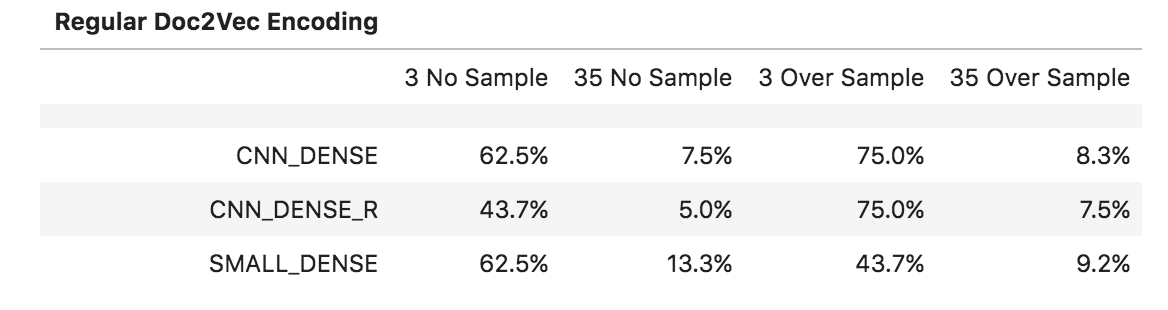
\includegraphics[width=0.5\textwidth]{regular_Doc2Vec}
     \caption{Summary of Author Predictions Using Doc2Vec}
   \end{figure}

This is the original set of tests we ran once we starting getting some
more stable results. You will notice the CNN layers prove to outperform
our custom encoding method. It is especially true when oversampling is
in play. With so few authors being trained on, having duplicate data
helps it learn those authors better, even though it may be overfitting.

.. raw:: latex

   \begin{figure}[h!]
     \centering
       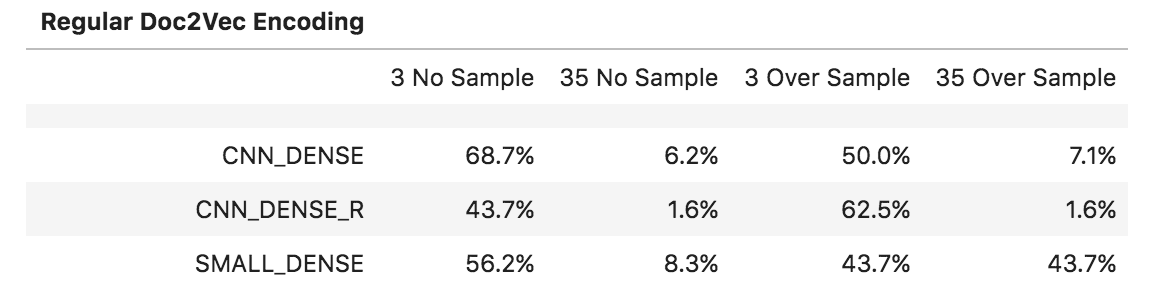
\includegraphics[width=0.5\textwidth]{reversed_Doc2Vec}
     \caption{Summary of Author Predictions Using Reversed Sentence Encoding with Doc2Vec}
   \end{figure}

This is a slightly modified encoding of our author and review data. The
sentences in each review are reversed. This encoding caused the
Convolutional networks to perform terribly when oversampling was used.
Even our custom encoding did alright as long as the sampling was normal.
Having three authors proved to be the best given normal sampling as
well.

.. raw:: latex

   \begin{figure}[h!]
     \centering
       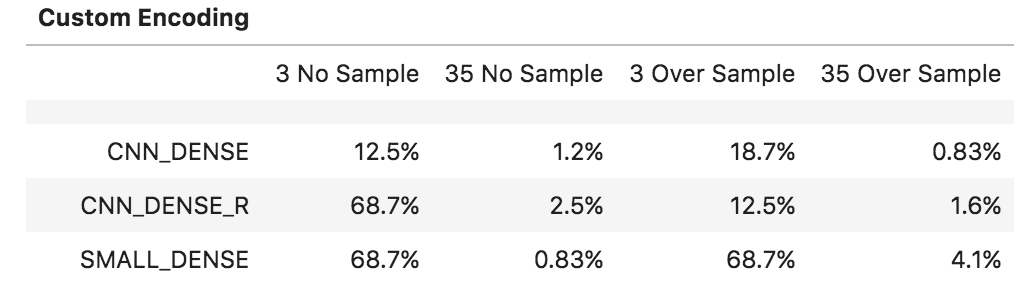
\includegraphics[width=0.45\textwidth]{custom}
     \caption{Summary of Author Prediction Using our Custom Encoding}
   \end{figure}

Our custom encoding performed worst of all when trying to determine
authorship. The only parameters that resulted in good performance were
having three authors and keeping the normal sample size. The Dense
network actually performed better overall than the Convolutional
networks using our own encoding.

Out of every encoding we tried, the regular Doc2Vec encoding in Fig.1
worked the best in terms of detecting correct authorship. Fig.3 end up
having the worst performance among the networks. And, of course, the
Doc2Vec model using reversed sentences was somewhere inbetween.

.. raw:: latex

   \begin{figure}[h!]
     \centering
       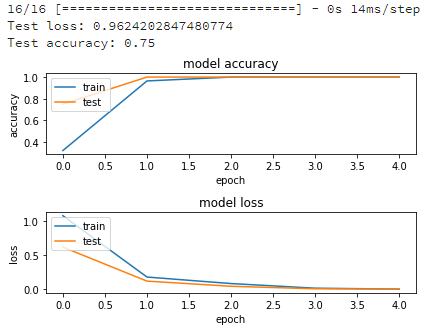
\includegraphics[width=0.45\textwidth]{CNN_DENSE_OVERSAMPLING_RESULTS_3_AUTHORS}
     \caption{Accuracy and Loss for CNN\_DENSE with three Authors with Normal Sampling}
   \end{figure}

.. raw:: latex

   \begin{figure}[h!]
     \centering
       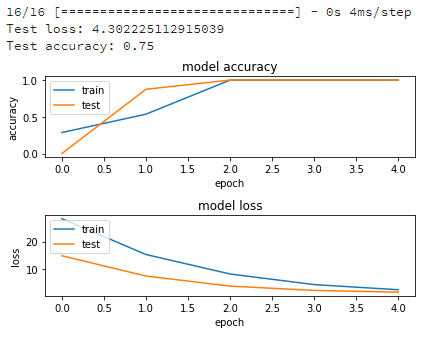
\includegraphics[width=0.45\textwidth]{CNN_DENSE_3_REGULARIZERS_OVERSAMPLING_RESULTS}
     \caption{Accuracy and Loss for CNN\_DENSE\_R with three Authors with 3x Sampling}
   \end{figure}

Fig.4 and Fig.5 show the two best classifications among every network
and encoding scheme. The both come from Fig.1 which has the Doc2Vec
encodings with normal sentence structure. You will notice pretty quickly
some overfitting is occurring. Especially since there are only three
authors the net is training on in these example runs.

.. raw:: latex

   \begin{figure}[h!]
     \centering
       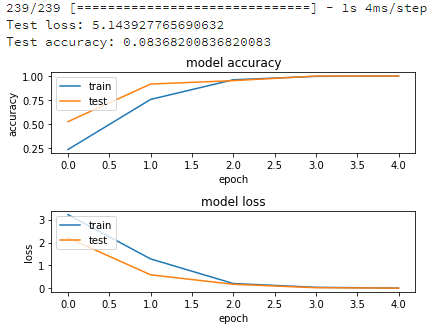
\includegraphics[width=0.45\textwidth]{CNN_DENSE_OVERSAMPLING_RESULTS_35_AUTHORS}
     \caption{Accuracy and Loss for CNN\_DENSE with three Authors with 3x Sampling}
   \end{figure}

In Fig.6 , you can see it performs the worst at only a fraction of a
single percent. In this case, both our custom encoding and the regular
sentences with Doc2Vec performed equally poor. The testing accuracy is
stagnant and just stays in a platuae the entire time. The training
accuracy spikes up quickly which means overfitting is happening

% DISCUSSION SECTION
\section{Discussion and Conclusion}

    In general, our tests along with our neural networks, proved to be mostly unsuccessful at building a unique feature-set for classifying individual authors. The best result that was achieved (referenced above in Fig.5 and Fig.6) was only acheivable using three authors. As the number of authors increased, the accuracy decreased sharply. Overfitting was a huge problem proving to be our biggest downfall. After around 5-10 epochs, the loss goes down to zero (or very close to) and the accuracy shoots up to one. Even in our custom encoding, it overfits to the first author everytime a prediction occurs. This is because the first author has many more reviews in the dataset. It becomes tailored to the auther who has more data points. In the future, finding evenly ditributed datasets would probably be more helpful. Along with that, Word2Vec and Doc2Vec are not the best at picking up stylistic differences in an individual author. They are mostly adept at finding semantic similarites instead of these unique writing styles. If we had increased the width of these word vectors, they could've been more unique. Though 300 is the standard, more would produce even more unique representations of document-level data. Removing all alpha-numeric characters may have affected it as well. Maybe knowing the context via punctuation would've proven useful to training the model in Word2Vec and Doc2Vec. Even making punction its own word may have proven useful. In general, we needed more than semantics to determine the style of an auther to fully be able to predict similiarities.\cite{b5}

% REFERENCES
% THIS IS CREATED AUTOMATICALLY
\bibliographystyle{IEEEtran}
\bibliography{References} % change if another name is used for References file

\end{document}
